\subsubsection{Chosen method}
To estimate the localization of sources, beamforming technique is dismissed in favour of time-delay of arrival (TDOA) method. This is the only feasible method for this case, as beamforming cannot be used when distance between sensors is large. In addition, it is computationally cheaper and uses time signal processing and estimation theory.

TDOA should not be confused with TDE, although here both terms will be used with no distintion. TDE is in general the estimation of the delay of two signals, and can be split in two categories: TOA and TDOA. The former deals with the time difference from the emission of a known signal from the transmitter of a device until the reflection of this signal on the target comes back at the receiver. On the other hand, TDOA tries to estimate the delay of an incoming signal in two separated receivers. This signals is solely produced by the target. As the receivers (in our case hydrophones) are at different positions, the signal that impinges on one sensor would be a shifted version of the one at the other sensor. In this article we will focus on the second case: TDOA. Passive (just listening) is preferable in front of active approaches such as SONAR or beamforming techniques, because of ecological and technical aspects: the microphones used in the available data were separated many kilometers away from each other.

\subsubsection{Cons to face}
The passive TDOA approach and the underwater environment imply some inconvenients that must be taken into consideration:
\begin{enumerate}
  \item The incoming signal is totally unknown, in contrast of in active (TOA) approach, where a simple matched filter would be optimum when the reference signal is produced by us. In our case, TDOA can do no presumption of the waveform, excluding the frequency range. Minke whales usally emit sounds from 1 to \SI{12}{\kilo\Hz}.
  \item Signal to noise ratio (SNR) is very low. This will be the main limitation and that's the reason of the emphasis on the prefiltering methods for noise reduction.
  \item Correlated noise, as the main contribution to it is not white noise, but strong interferences from other animals, devices and water currents.
  \item Reflections on the water surface, mainly. This can make the algorithm to get confused by them and could return a wrong result. Reflections on the seafloor are negligible, as hydrophones are usually placed very near to the ground.
  \item The recordings will not be just a shifted version of the other ones. Noise, reflections and interferences will introduce huge bias and variance in the estimation if not treated correctly.
  \item Sources (whales) will not be still, so the delay will not be a constant in the long-run.
\end{enumerate}

\vspace{5pt}
\subsubsection{Signal model}
  As stated before, the overall results should take into consideration far reflections on the ocean surface. A simple scheme is shown in Figure \ref{fig:reflections}, where flat ground is assumed.  

  \vspace{5pt}
  \begin{figure}[htb]
	  \begin{center}
		  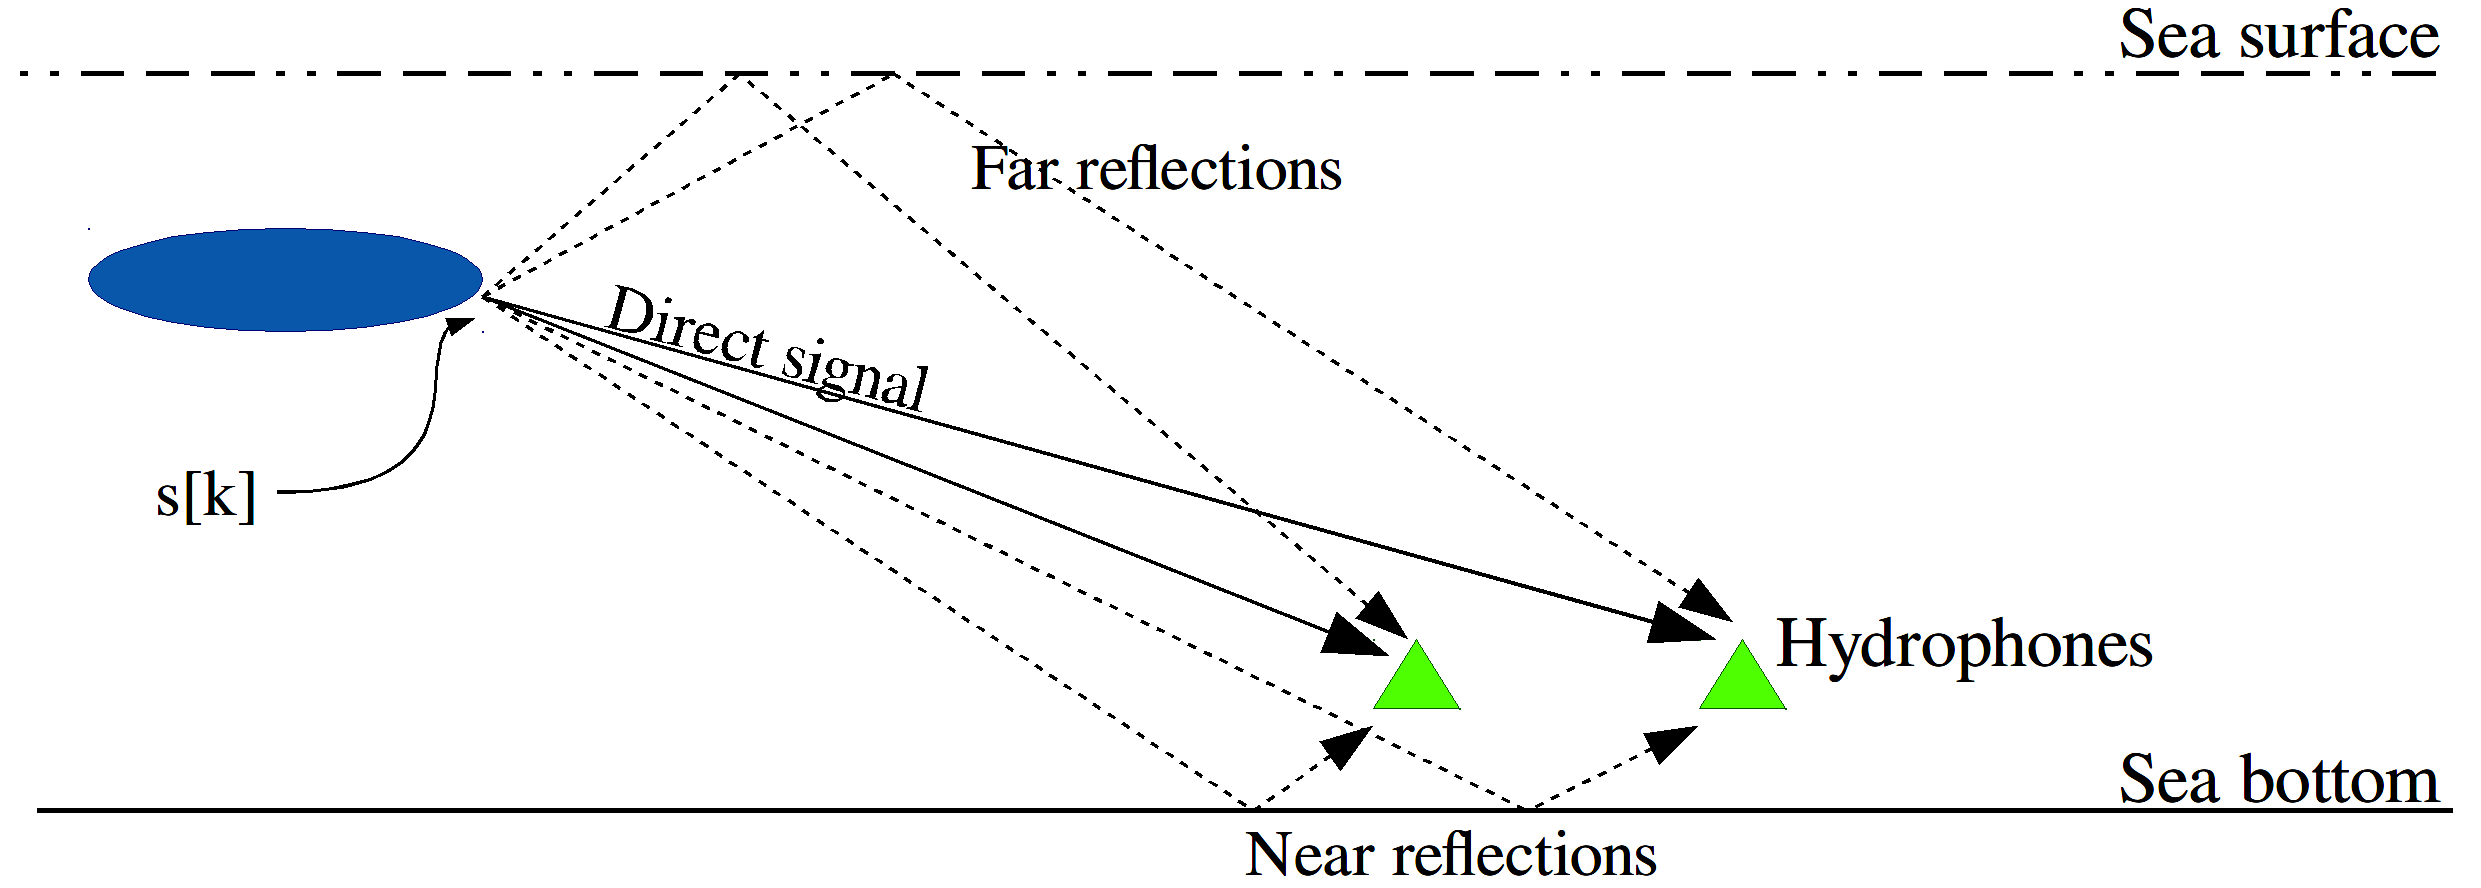
\includegraphics[width=0.5\textwidth]{figures/model.png}
	  \end{center}
	  \caption{Reflections in an underwater environment}
	  \label{fig:reflections}
  \end{figure}
  
  Received signal could be expressed in general as
  $$ r_1[n] = h_1[n]^T s[n] + w_1[n] $$
  $$ r_2[n] = h_2[n]^T s[n] + w_2[n] $$
  
  In an ideal case, $h_k[n]$ would be a Kronecker delta at the delay position, so $h_k[n] = [0\ 0\ ...\ \alpha\ ...\ 0\ 0]$, but in general, as indicated in the fifth con to face, distorsion and reflections can make the impulse response of the channel to be any kind \cite{overview}.
  $$ h_k[n] = [h_0\ h_1\ ...\ h_{L-1}] $$
  
